\RequirePackage[orthodox]{nag}
\documentclass[11pt]{article}

%% Define the include path
\makeatletter
\providecommand*{\input@path}{}
\g@addto@macro\input@path{{include/}{../include/}}
\makeatother

\usepackage{../../include/akazachk}


\title{ECH4905 ChemE Optimization HW 4}
\author{Andres Espinosa}

\begin{document}
\maketitle

\section{Problem 1}
Consider the following integer programming problem:


\begin{align*}
  \text{maximize} & \quad 1.2y_1 + y_2 \\
  \text{subject to} & \quad y_1 + y_2 \leq 1 \\
  & \quad 1.2y_1 + 0.5y_2 \leq 1 \\
  & \quad y_1, y_2 \in \{ 0,1 \}
\end{align*}

\subsection{Part a}
\label{prob1parta}
Solve the first relaxed LP subproblem by hand using the simplex method and derive Gomory cuts based on the LP relaxation.

\textbf{Solution:} To tackle this problem we first relax the problem and then turn the problem above into the standard form so we can create a simplex tableau from it.

\begin{align*}
    \text{maximize} & \quad 1.2y_1 + y_2 \\
    \text{subject to} & \quad y_1 + y_2 + s_1= 1 \\
    & \quad 1.2y_1 + 0.5y_2 + s_2 = 1 \\
    & \quad y_1 + s_3 = 1 \\
    & \quad y_2 + s_4 = 1 \\
    & \quad y_1, y_2, s_1, s_2, s_3, s_4 \geq 0
\end{align*}

In matrix notation,
\begin{align*}
  \text{minimize} & \quad \textbf{c}^\top \textbf{x} \\
  \text{subject to} & \quad \textbf{A} \textbf{x} = \textbf{b} \\
  & \quad \textbf{x} \succeq 0
\end{align*}
where
\begin{align*}
    \textbf{c} = 
  \begin{bmatrix}
     -1.2 \\ -1 \\ 0 \\ 0 \\ 0 \\ 0
  \end{bmatrix}, \quad
  \textbf{A} = 
  \begin{bmatrix}
    1 & 1 & 1 & 0 & 0 & 0 \\
    1.2 & 0.5 & 0 & 1 & 0 & 0 \\
    1 & 0 & 0 & 0 & 1 & 0 \\
    0 & 1 & 0 & 0 & 0 & 1
  \end{bmatrix}, \quad
  \textbf{b} = 
  \begin{bmatrix}
    1 \\ 1 \\ 1 \\ 1
  \end{bmatrix}, \quad
  \textbf{x} = 
  \begin{bmatrix}
    y_1 \\ y_2 \\ s_1 \\ s_2 \\ s_3 \\ s_4
  \end{bmatrix}
\end{align*}
(with a flipped objective component)

The initial simplex tableau for the problem is as follows:

\[
\begin{array}{c|cccccc|c|c}
\text{Basic Var} & y_1 & y_2 & s_1 & s_2 & s_3 & s_4 & \text{RHS} & \alpha \\
\hline
s_1 & 1 & 1 & 1 & 0 & 0 & 0 & 1 &  \\
s_2 & 1.2 & 0.5 & 0 & 1 & 0 & 0 & 1 &  \\
s_3 & 1 & 0 & 0 & 0 & 1 & 0 & 1 &  \\
s_4 & 0 & 1 & 0 & 0 & 0 & 1 & 1 &  \\
\hline
\text{obj} & -1.2 & -1 & 0 & 0 & 0 & 0 & - & - \\
\end{array}
\]
we can define the slack variables equal to the right hand side, and this is in turn a basic feasible solution, so we can jump into phase 2.

We select the $y_1$ as the entering variable and calculate the alpha value for each basic variable
\[
\begin{array}{c|cccccc|c|c}
\text{Basic Var} & y_1 & y_2 & s_1 & s_2 & s_3 & s_4 & \text{RHS} & \alpha \\
\hline
s_1 & 1 & 1 & 1 & 0 & 0 & 0 & 1 & \frac{1}{1} \\
s_2 & 1.2 & 0.5 & 0 & 1 & 0 & 0 & 1 & \frac{1}{1.2} \\
s_3 & 1 & 0 & 0 & 0 & 1 & 0 & 1 & \frac{1}{1} \\
s_4 & 0 & 1 & 0 & 0 & 0 & 1 & 1 & \frac{1}{0} \\
\hline
\text{obj} & -1.2 & -1 & 0 & 0 & 0 & 0 & - & - \\
\end{array}
\]
We pivot this on the 1st column ($y_1$) and the 2nd row ($s_2$)
\[
\begin{array}{c|cccccc|c|c}
\text{Basic Var} & y_1 & y_2 & s_1 & s_2 & s_3 & s_4 & \text{RHS} & \alpha \\
\hline
s_1 & 0 & \frac{7}{12} & 1 & -\frac{5}{6} & 0 & 0 & \frac{1}{6} &  \\
y_1 & 1 & \frac{5}{12} & 0 & \frac{5}{6} & 0 & 0 & \frac{5}{6} &  \\
s_3 & 0 & -\frac{5}{12} & 0 &  -\frac{5}{6} & 1 & 0 & \frac{1}{6} &  \\
s_4 & 0 & 1 & 0 &  0 & 0 & 1 & 1 &  \\
\hline
\text{obj} & 0 & -0.5 & - & - & - & - & - & - \\
\end{array}
\]
With blands rule, we pick $y_2$ and calculate the alpha value for each basic variable.
\[
\begin{array}{c|cccccc|c|c}
\text{Basic Var} & y_1 & y_2 & s_1 & s_2 & s_3 & s_4 & \text{RHS} & \alpha \\
\hline
s_1 & 0 & \frac{7}{12} & 1 & -\frac{5}{6} & 0 & 0 & \frac{1}{6} & \frac{2}{7} \\
y_1 & 1 & \frac{5}{12} & 0 & \frac{5}{6} & 0 & 0 & \frac{5}{6} & \frac{2}{1} \\
s_3 & 0 & -\frac{5}{12} & 0 &  -\frac{5}{6} & 1 & 0 & \frac{1}{6} & -\frac{1}{5} \\
s_4 & 0 & 1 & 0 &  0 & 0 & 1 & 1 & \frac{1}{1} \\
\hline
\text{obj} & 0 & -0.5 & - & - & - & - & - & - \\
\end{array}
\]
We pivot on the 2nd column ($y_2$) and the 1st row ($s_1$).
\[
\begin{array}{c|cccccc|c|c}
\text{Basic Var} & y_1 & y_2 & s_1 & s_2 & s_3 & s_4 & \text{RHS} & \alpha \\
\hline
y_2 & 0 & 1 & \frac{12}{7} & -\frac{10}{7} & 0 & 0 & \frac{2}{7} &  \\
y_1 & 1 & 0 & -\frac{5}{7} & \frac{60}{42} & 0 & 0 & \frac{30}{42} &  \\
s_3 & 0 & 0 & \frac{5}{7} &  -\frac{60}{42} & 1 & 0 & \frac{12}{42} &  \\
s_4 & 0 & 0 & -\frac{12}{7} &  \frac{60}{42} & 0 & 1 & \frac{30}{42} &  \\
\hline
\text{obj} & 0 & 0 & 0.857 & 0.286  & 0 & 0 & 0 & -1.143 \\
\end{array}
\]
This is the optimal solution to the LP relaxed problem.
Now we will derive Gomory cuts from this LP relaxed problem.
Since each constraint has a non-integer solution, we can generate a Gomory cut on each constraint.

\begin{align*}
  y_2 + \text{floor}(\frac{12}{7}) s_1 + \text{floor}(\frac{-10}{7}) s_2 \leq \text{floor}(\frac{2}{7}) \\
  y_1 + \text{floor}(\frac{-5}{7}) s_1 + \text{floor}(\frac{10}{7}) s_2 \leq \text{floor}(\frac{5}{7}) \\
  s_3 + \text{floor}(\frac{5}{7}) s_1 + \text{floor}(\frac{-10}{7})s_2 \leq \text{floor}(\frac{2}{7}) \\
  s_4 + \text{floor}(\frac{-12}{7}) s_1 + \text{floor}(\frac{10}{7}) s_2 \leq \text{floor}(\frac{5}{7})
\end{align*}
These turn into the cuts
\begin{align*}
  y_2 + s_1 -2 s_2 \leq 0 \\
  y_1 - s_1 + s_2 \leq 0 \\
  s_3 -2 s_2 \leq 0 \\
  s_4 -2 s_1 + s_2 \leq 0
\end{align*}

\subsection{Part b}
Solve the above problem with the branch and bound method by enumerating nodes in the tree and solving the LP subproblems using GAMS.

\textbf{Solution: }
The initial LP relaxed problem is solved in \ref{prob1parta}, so we can start with the parent node.
An important note for this question, I will be solving the LPs in my custom \texttt{gatorpy} LP solver so that I can use them as verification tests.
The code used will be available in section \ref{problem1code}
\begin{center}
  \begin{adjustbox}{width=0.5\textwidth}
  \begin{tikzpicture}[
    level 1/.style={sibling distance=80mm},
    level 2/.style={sibling distance=35mm},
    level distance=3.5cm,
    edge from parent/.style={draw, -latex, very thick},
    every node/.style={draw, rounded corners, text width=5cm, align=center, very thick, font=\small}
]
    
% Root node
\node {
  \begin{align*}
      & [\frac{5}{7},  \frac{2}{7},0,0,\frac{2}{7},\frac{5}{7}], z = \frac{8}{7} \\
      & \text{maximize} \quad 1.2y_1 + y_2 \\
      & \text{subject to} \quad y_1 + y_2 + s_1 = 1, \\
      & \quad 1.2y_1 + 0.5y_2 + s_2 = 1, \\
      & \quad y_1 + s_3 = 1, \\
      & \quad y_2 + s_4 = 1, \\
      & \quad y_1, y_2, s_1, s_2, s_3, s_4 \geq 0. \\
      & UB= \frac{8}{7}, LB = -inf
  \end{align*}
};
\end{tikzpicture}
\end{adjustbox}
\end{center}
Since all variables are fractional, we can pick the first one $y_1$ to branch on
\begin{center}
  \begin{adjustbox}{width=0.8\textwidth}
  \begin{tikzpicture}[
    level 1/.style={sibling distance=100mm},
    level 2/.style={sibling distance=80mm},
    level distance=10cm,
    edge from parent/.style={draw, -latex, very thick},
    every node/.style={draw, rounded corners, text width=5cm, align=center, very thick, font=\small}
]
    
% Root node
\node {
  \begin{align*}
      & [\frac{5}{7},  \frac{2}{7},0,0,\frac{2}{7},\frac{5}{7}], z = \frac{8}{7} \\
      & \text{maximize} \quad 1.2y_1 + y_2 \\
      & \text{subject to} \quad y_1 + y_2 + s_1 = 1, \\
      & \quad 1.2y_1 + 0.5y_2 + s_2 = 1, \\
      & \quad y_1 + s_3 = 1, \\
      & \quad y_2 + s_4 = 1, \\
      & \quad y_1, y_2, s_1, s_2, s_3, s_4 \geq 0. \\
      & UB= \frac{8}{7}, LB = -inf
  \end{align*}
}
    % Left child of Root
    child {node {
      \begin{align*}
          & [0, 1], z = 1 \\
          & \text{maximize} \quad 1.2y_1 + y_2 \\
          & \text{subject to} \quad y_1 \leq 0, \\
          & \quad y_1 + y_2 \leq 1, \\
          & \quad 1.2y_1 + 0.5y_2 \leq 1, \\
          & \quad y_1 \leq 1, \\
          & \quad y_2 \leq1, \\
          & \quad y_1, y_2 \geq 0. \\
          & UB= \frac{8}{7}, LB = 1, optimal
      \end{align*}
    }
    edge from parent node[draw=none, pos=0.5, above left] {$y_1 = 0$}}
    % Right child of Root
    child {node {
      \begin{align*}
          & [1, 0], infeasible \\
          & \text{maximize} \quad 1.2y_1 + y_2 \\
          & \text{subject to} \quad y_1 \geq 1, \\
          & \quad y_1 + y_2 \leq 1, \\
          & \quad 1.2y_1 + 0.5y_2 \leq 1, \\
          & \quad y_1 \leq 1, \\
          & \quad y_2 \leq1, \\
          & \quad y_1, y_2 \geq 0. \\
          & pruned
      \end{align*}
    }
    edge from parent node[draw=none, pos=0.5, above right] {$y_1 = 1$}};
\end{tikzpicture}
\end{adjustbox}
\end{center}

Via the branch and bound method, the optimal solution to the problem
\begin{align*}
  \text{maximize} & \quad 1.2y_1 + y_2 \\
  \text{subject to} & \quad y_1 + y_2 \leq 1 \\
  & \quad 1.2y_1 + 0.5y_2 \leq 1 \\
  & \quad y_1, y_2 \in \{ 0,1 \}
\end{align*}
is $y_1=0,y_2=1,z=1$.

\clearpage
\section{Problem 2}
\label{prob2}

Consider the following superstructure for the separation of four chemical components using sharp distillation columns. 
\begin{figure}[htbp]
  \centerline{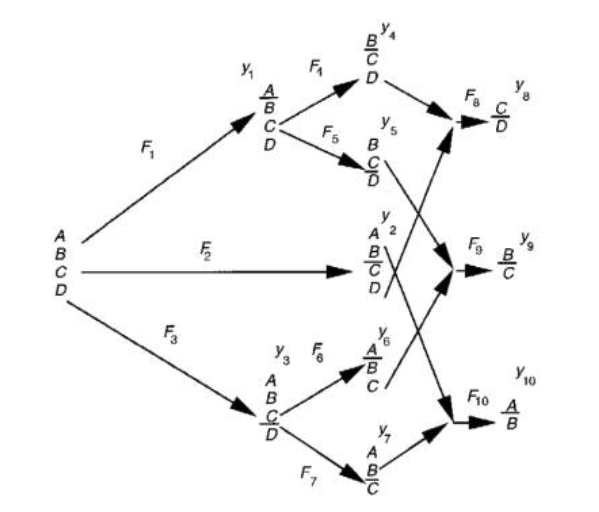
\includegraphics[width=0.50\textwidth]{images/prob2_superstructure.png}}
  \caption{Problem 2 superstructure}
  \label{fig:prob2_superstructure}
\end{figure}
The total cost of a distillation column is calculated as follows:

\[
\text{cost}_k = \alpha_k + \beta_k F_k + \gamma_\text{Hot} Q_k^\text{Hot} + \gamma_\text{Cold} Q_k^\text{Cold}
\]

where:
\begin{itemize}
  \item $\alpha_k$ represents a fixed capital cost,
  \item $\beta_k$ represents the variable investment cost,
  \item $\gamma_{\text{Hot}/\text{Cold}}$ is the cost of hot/cold utilities, and
  \item $Q_k^\text{Hot}/Q_k^\text{Cold}$ is the total demand of hot and cold utilities (assumed to be equal).
\end{itemize}

Given:
\begin{itemize}
  \item Initial feed: 1000 Kmol/h,
  \item Feed composition (mole fraction): A = 0.15, B = 0.3, C = 0.35, D = 0.2.
\end{itemize}
and the following data:
\begin{figure}[htbp]
  \centerline{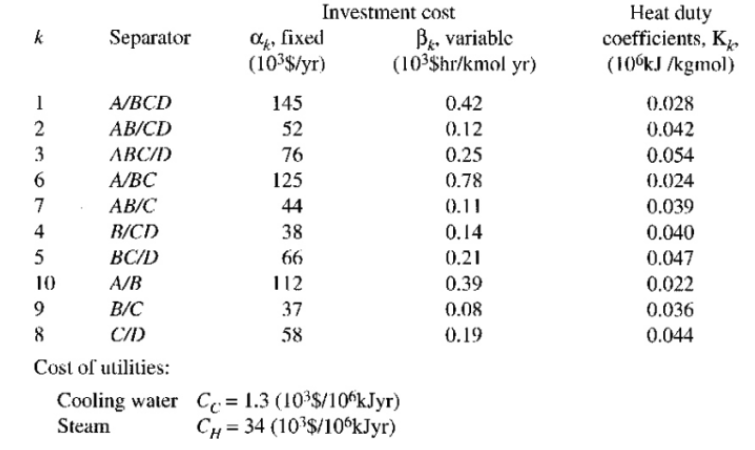
\includegraphics[width=0.75\textwidth]{images/prob2_table.png}}
  \caption{Problem 2 Data}
  \label{fig:prob2_table}
\end{figure}

\subsection{Part A: MILP Formulation}
Formulate a Mixed-Integer Linear Programming (MILP) problem to find the optimal sequence of distillation columns. 
Identify at least 2 logicx based equations that can be formulated to tighten the problem formulation.

\textbf{Solution:}
In order to solve this problem, I will first identify the variables and model the binary flow and decision logic.
Then, I will attempt to solve the problem while ignoring the Hot/Cold variables since I am much less confident on implementing that than the other sections.
After getting a solution working while ignoring the hot/cold components, I will then implement those $\gamma, Q$ parameters into the problem.

\subsubsection{Binary logic}
To solve this, I will start by creating a series of statements that must be true for this flow to work.
I will be using the same $y$ variables for each distillation column that can be seen in the superstructure diagram \ref{fig:prob2_superstructure}.
\begin{itemize}
  \item One of $y_1,y_2,y_3$ must be chosen.
  \item If $y_1$ is chosen, then either $y_4$ xor $y_5$ must be chosen.
  \item If $y_2$ is chosen, then both $y_8$ and $y_{10}$ must be chosen.
  \item If $y_3$ is chosen, then either $y_6$ xor $y_7$ must be chosen.
  \item If $y_4$ is chosen, then $y_8$ must be chosen.
  \item If $y_5$ is chosen, then $y_9$ must be chosen.
  \item If $y_6$ is chosen, then $y_9$ must be chosen.
  \item If $y_7$ is chosen, then $y_{10}$ must be chosen.
\end{itemize}
I believe this to be a sufficient set of logic statements to model the problem of choosing a distillation problem.
Getting rid of the implications:
\begin{itemize}
  \item One of $y_1,y_2,y_3$ must be chosen.
  \item $y_1=0$ or either $y_4$ xor $y_5$ must be chosen.
  \item $y_2=0$ or both $y_8$ and $y_{10}$ must be chosen.
  \item $y_3=0$ or either $y_6$ xor $y_7$ must be chosen.
  \item $y_4=0$ or $y_8$ must be chosen.
  \item $y_5=0$ or $y_9$ must be chosen.
  \item $y_6=0$ or $y_9$ must be chosen.
  \item $y_7=0$ or $y_{10}$ must be chosen.
\end{itemize}
We can then translate these second parts into different clauses
\begin{align*}
  \text{One of $y_1,y_2,y_3$ must be chosen.} & \quad \rightarrow & y_1 + y_2 + y_3 = 1 \\
  \text{Either $y_4$ xor $y_5$ must be chosen.} & \quad \rightarrow & y_4 + y_5 = 1 \\
  \text{both $y_8$ and $y_{10}$ must be chosen.} & \quad \rightarrow & y_8 =1 \cap y_{10} = 1  \\
  \text{Either $y_6$ xor $y_7$ must be chosen.} & \quad \rightarrow & y_6 + y_7 = 1 \\
  \text{$y_8$ must be chosen.} & \quad \rightarrow & y_8 = 1 \\
  \text{$y_9$ must be chosen.}& \quad \rightarrow & y_9 = 1 \\
  \text{$y_9$ must be chosen.} & \quad \rightarrow & y_9 = 1 \\
  \text{$y_{10}$ must be chosen.} & \quad \rightarrow & y_{10} =1
\end{align*}
which can in turn be converted to
\begin{align*}
  y_1 + y_2 + y_3 = 1 \\
  y_1 = 0 & \cup y_4 + y_5 = 1 \\
  y_2 = 0 & \cup (y_8 =1 \cap y_{10} = 1)  \\
  y_3 = 0 & \cup y_6 + y_7 = 1 \\
  y_4 = 0 & \cup y_8 = 1 \\
  y_5 = 0 & \cup y_9 = 1 \\
  y_6 = 0 & \cup y_9 = 1 \\
  y_7 = 0 & \cup y_{10} =1
\end{align*}
We can subtract each variable on the left from 1 so we can add them together and distribute the and operation out for the third.
\begin{align*}
  y_1 + y_2 + y_3 = 1 \\
 ( 1-y_1 = 1) & \cup( ((y_4=1)\cup (y_5=1)) \cap ((1-y_4=1)\cup (1-y_5=1))) \\
 (( 1-y_2 = 1) \cup (y_8 = 1)) & \cap ( ( 1-y_2 = 1) \cup (y_{10} = 1))  \\
( 1-y_3 = 1) & \cup( ((y_6=1)\cup (y_7=1)) \cap ((1-y_6=1)\cup (1-y_7=1))) \\
  1-y_3 = 1 & \cup y_6 + y_7 = 1 \\
  1-y_4 = 1 & \cup y_8 = 1 \\
  1-y_5 = 1 & \cup y_9 = 1 \\
  1-y_6 = 1 & \cup y_9 = 1 \\
  1-y_7 = 1 & \cup y_{10} =1
\end{align*}
We turn this into the equivalent equations
\begin{align*}
  y_1 + y_2 + y_3 = 1 \\
  (1-y_1 = 1) &\cup ((y_4=1\cup y_5=1))\\
  (1-y_1 = 1) &\cup ((1-y_4=1)\cup (1-y_5=1)) \\
  1-y_2 + y_8 \geq 1 \\
  1-y_2 + y_{10} \geq 1 \\
  (1-y_3 = 1) & \cup (y_6=1\cup y_7=1) \\
  (1-y_3 = 1) & \cup ((1-y_6=1)\cup (1-y_7=1)) \\
  1-y_4 + y_8 \geq 1 \\
  1-y_5+ y_9 \geq 1 \\
  1-y_6 + y_9 \geq 1 \\
  1-y_7 + y_{10} \geq 1
\end{align*}

Finally, we can bring them all into pure math below
\begin{align*}
  y_1 + y_2 + y_3 = 1 \\
  1-y_1 + y_4 + y_5 \geq 1 \\
  1-y_1 + 1-y_4 + 1-y_5 \geq 1 \\
  1-y_2 + y_8 \geq 1 \\
  1-y_2 + y_{10} \geq 1 \\
  1-y_3 + y_6 + y_7 \geq 1 \\
  1-y_3 + 1 - y_6 + 1- y_7 \geq 1 \\
  1-y_4 + y_8 \geq 1 \\
  1-y_5+ y_9 \geq 1 \\
  1-y_6 + y_9 \geq 1 \\
  1-y_7 + y_{10} \geq 1
\end{align*}
Note: These equations are not completely sufficient on themselves, they require that each distillation column has a non-negative cost component.
Otherwise, it could be possible for $y_8$ and $y_7$ to be chosen, but it isn't necessary since the optimization should only yield a solution where distillation columns are used if they are needed to.
\subsection{Model w/o HotCold}
After having solved the binary logic problems above, I will start by denoting the parameters for the model.
This model is actually not too bad (unless I am missing the importance of the feed composition asides from flow removal).

\textit{Parameters:}
This problem has a feed composition parameter set $f_A=0.15,f_B,0.30,f_C=0.35,f_D=0.2$. 
(Important note: I am using $x$ for the flow, so $f$ is a parameter for feed composition).
There is the input supply $S=1000$.
Fixed capital cost $\alpha_k$ for each $k \in [1,\dots,10]$ distillation column and variable cost $\beta_k$.

\textit{Variables:}
I am using the continuous variables $x_i \in [1,\dots,13]$ to represent the flow from column to column.
Below is a table that maps the variable index to each flow
\begin{table}[htbp]
\centering
\begin{tabular}{|c|c|}
\hline
\textbf{Index} & \textbf{Flow Description} \\ \hline
1 & Feed to Column 1 \\ \hline
2 & Feed to Column 2 \\ \hline
3 & Feed to Column 3 \\ \hline
4 & Output from Column 1 to Column 4 \\ \hline
5 & Output from Column 1 to Column 5 \\ \hline
6 & Output from Column 2 to Column 6 \\ \hline
7 & Output from Column 2 to Column 7 \\ \hline
8 & Output from Column 4 to Column 8 \\ \hline
9 & Output from Column 5 to Column 9 \\ \hline
10 & Output from Column 6 to Column 9 \\ \hline
11 & Output from Column 7 to Column 10 \\ \hline
12 & Output from Column 8 to Final Product \\ \hline
13 & Output from Column 10 to Final Product \\ \hline
\end{tabular}
\caption{Mapping of variable indices to flow descriptions.}
\label{tab:flow_mapping}
\end{table}
I am also using variables $y_k$, $k \in [1,\dots,10]$ to denote the binary choice of using distillation column $k$.

\textit{Constraints:}
We can model our constraints as follows:
\begin{align*}
  y_k & \quad & \quad \text{See above for distillation constraints} \\
   e
\end{align*}


\subsection{Part B: Solve Using GAMS}
Solve the problem using GAMS.

\subsection{Part C: Integer Cut}
Once the solution is found:
\begin{itemize}
  \item Identify the active binary variables in the optimal solution.
  \item Formulate an integer cut to exclude this solution from the feasible space.
  \item Solve the problem again to find the next best solution.
\end{itemize}

\clearpage
\section{Problem 3}
\label{prob3}

Given are three candidate reactors for the reaction \( A \rightarrow B \), where we would like to produce 10 kmol/h of \( B \). Up to 15 kmol/hr of reactant \( A \) are available at a price of \$2/kmol. The data on the three reactors is as follows:

\begin{table}[htbp]
\centering
\begin{tabular}{|c|c|c|}
\hline
\textbf{Reactor} & \textbf{Conversion} & \textbf{Cost} \\ \hline
1 & 0.8 & \( 8 + 1.5 \cdot \text{Feed} \) \\ \hline
2 & 0.667 & \( 5.4 + \text{Feed} \) \\ \hline
3 & 0.555 & \( 2.7 + 0.5 \cdot \text{Feed} \) \\ \hline
\end{tabular}
\caption{Reactor Data}
\label{tab:reactor_data}
\end{table}

\subsection{Part A: Superstructure Design}
Design a superstructure to represent this problem.

\textbf{Solution:}
\begin{figure}[htbp]
\centering
\begin{tikzpicture}[
  node distance=2cm and 3cm,
  every node/.style={draw, circle, minimum size=1cm, align=center},
  every path/.style={draw, -latex, thick}
]

% Nodes
\node (A) {A};
\node[below left=of A] (R1) {Reactor 1};
\node[below=of A] (R2) {Reactor 2};
\node[below right=of A] (R3) {Reactor 3};
\node[below=of R1] (B1) {B};
\node[below=of R2] (B2) {B};
\node[below=of R3] (B3) {B};

% Paths
\path (A) -- (R1);
\path (A) -- (R2);
\path (A) -- (R3);
\path (R1) -- (B1);
\path (R2) -- (B2);
\path (R3) -- (B3);

\end{tikzpicture}
\caption{Superstructure for the reaction \( A \rightarrow B \) with three reactors.}
\label{fig:superstructure_reactors}
\end{figure}
Not sure if I am oversimplifying this.
This superstructure assumes that no A is recycled back into the reactor, and we only choose one reactor.
This is generally a simple problem, we are effectively picking which reactor to use to minimize the cost.

\subsection{Part B: MILP Formulation}
Determine a MILP formulation.

\textbf{Solution:}
In order to solve this MILP formulation, I will start thinking about this in a GAMS/modeling language way starting with parameters.

\textit{Parameters:} 
We have parameters $k_i$ as the $A \rightarrow B$ conversion of reactor $i$.
We also have cost components $d_i$ as the constant cost of using reactor $i$ and $c_i$ as the multiplicative cost of feeding $A$ through reactor $i$.
Our demand parameter $D$ for the amount of B we would like to produce and our supply $S$ that we have available.
We can also have the price of using a kmol of $A$ as $p$.
Below are the numerical representations of the problem parameters:
\begin{align*}
  k_1=\frac{4}{5}, k_2=\frac{2}{3}, k_3=\frac{5}{9} \\
  d_1=8, d_2=5.4, d_3=2.7; c_1=1.5, c_2=1, c_3=0.5 \\
  D = 10, S=15, p=2
\end{align*}
\textit{Variables:}
Our variables for this problem are as follows:
We have $x_{i}$ as the amount of $A$ delivered to the $i$-th reactor.
In order to model our decision to pick a reactor, we have variables $y_i$ which are booleans that signify if reactor $i$ has been chosen.

\textit{Constraints:}
We can model our constraints as follows:
\begin{align*}
  x_i \leq S, & \quad \forall i \in [1,2,3] & \quad \text{Supply Constraint} \\
  \sum_{i=1}^{3} k_i x_i \geq D & \quad & \quad \text{Demand Constraint} \\
  \sum_{i=1}^{3} y_i = 1 & \quad & \quad \text{One Reactor Constraint} \\
  x_i \leq S y_i, & \quad \forall i \in [1,2,3] & \quad \text{Big-M One Reactor Flow Constraint} \\
  x_i \geq 0, & \quad \forall i \in [1,2,3] & \quad \text{Non-negativity} \\
  y_i \in \{ 0,1 \}  & \quad \forall i \in [1,2,3] & \quad \text{Binaries}
\end{align*}

We can also get rid of the supply constraint since the Big-M naturally handles that.
The GAMS solution below drops the supply constraint.
\textit{Objective:}
Our objective in this problem is to minimize the cost while still meeting the demand.
We can bunch these costs into different components

\begin{align*}
  p\sum_{i=1}^{3}x_i  & \quad \text{Supply component} \\
  \sum_{i=1}^{3}d_i y_i & \quad \text{Reactor constant component} \\
  \sum_{i=1}^{3}c_i y_i & \quad \text{Reactor processing component} \\
\end{align*}
\subsection{Part C: Solve Using GAMS}
Solve in GAMS.

\textbf{Solution:}
The optimal solution was found to be $x_1=12.5, y_1=1, z=34.5$, and the rest of the variables equal to 0.
GAMS code available in section \ref{problem3code}


\clearpage
\section{Code}
\subsection{Problem 1 Code}
\label{problem1code}
\begin{verbatim}
  # Parameters
  A_arr = np.array([[1,1],[1.2,0.5]])
  b_arr = np.array([1,1])
  c_arr = np.array([1.2,1])
  A = Parameter(A_arr)
  b = Parameter(b_arr)
  c = Parameter(c_arr)
  # Variables
  y = Variable(2)
  # Problem
  problem = Problem({
      'maximize': c.T @ y,
      'subject to': [
          A @ y <= b,
          y >= 0,
          y <= 1
      ]
  })
  
  # CVX Vars
  y_cvx = cp.Variable(2)
  # CVX Problem
  objective = cp.Maximize(c_arr @ y_cvx)
  constraints = [
      A_arr @ y_cvx <= b_arr,
      y_cvx >= 0,
      y_cvx <= 1
  ]
  problem_cvx = cp.Problem(objective, constraints)
  
  get_test_results(problem, problem_cvx, "HW5 Problem 1 initial LP relaxation")
  # branch and bound arrays
  I_y_1_arr = np.array([[1,0],[0,0]])
  I_y_2_arr = np.array([[0,0],[0,1]])
  I_y_1 = Parameter(I_y_1_arr)
  I_y_2 = Parameter(I_y_2_arr)
  # LEFT SPLIT
  # Problem
  problem = Problem({
      'maximize': c.T @ y,
      'subject to': [
          A @ y <= b,
          y >= 0,
          y <= 1,
          I_y_1 @ y <= 0,
      ]
  })
  
  # CVX Vars
  y_cvx = cp.Variable(2)
  # CVX Problem
  objective = cp.Maximize(c_arr @ y_cvx)
  constraints = [
      A_arr @ y_cvx <= b_arr,
      y_cvx >= 0,
      y_cvx <= 1,
      I_y_1_arr @ y_cvx <= 0
  ]
  problem_cvx = cp.Problem(objective, constraints)
  
  get_test_results(problem, problem_cvx, "HW5 Problem 1 Branch and Bound Left Split y_1 <= 0")
  
  # RIGHT SPLIT
  # Problem
  problem = Problem({
      'maximize': c.T @ y,
      'subject to': [
          A @ y <= b,
          y >= 0,
          y <= 1,
          I_y_1 @ y >= 1,
      ]
  })
  
  # CVX Vars
  y_cvx = cp.Variable(2)
  # CVX Problem
  objective = cp.Maximize(c_arr @ y_cvx)
  constraints = [
      A_arr @ y_cvx <= b_arr,
      y_cvx >= 0,
      y_cvx <= 1,
      I_y_1_arr @ y_cvx >= 1
  ]
  problem_cvx = cp.Problem(objective, constraints)
  
  get_test_results(problem, problem_cvx, "HW5 Problem 1 Branch and Bound Right Split y_1 >=1") 
  
  Test ID: HW5 Problem 1 initial LP relaxation
  CVX: (np.float64(1.14), array([[0.71, 0.29]]), True)
  GatORPy: (array(1.14285714), array([0.71428571, 0.28571429, 0.        , 0.        , 0.28571429,
         0.71428571]), True)
  Test passed: False 
  
  Test ID: HW5 Problem 1 Branch and Bound Left Split y_1 <= 0
  CVX: (np.float64(1.0), array([[0., 1.]]), True)
  GatORPy: (array(1.), array([0. , 1. , 0. , 0.5, 1. , 0. , 0. , 0. ]), True)
  Test passed: False 
  
  Test ID: HW5 Problem 1 Branch and Bound Right Split y_1 >=1
  CVX: (None, None, False)
  GatORPy: (array(0.8), array([ 1. , -0.4,  0.4,  0. ,  0. ,  1.4,  0. , -1. ]), True)
  Test passed: False 
\end{verbatim}




\subsection{Problem 3 Code}
\label{problem3code}
\begin{verbatim}
  GAMS 49.1.0  5c4d4ed6 Feb 15, 2025          DAX-DAC arm 64bit/macOS - 04/14/25 18:53:07 Page 1
G e n e r a l   A l g e b r a i c   M o d e l i n g   S y s t e m
C o m p i l a t i o n


   1  SETS
   2  i           'set of reactors'       /r1,r2,r3/
   3   
   4  ;
   5  Parameters
   6  k(i)    'conversion factors'    /r1 0.8, r2 0.666667, r3 0.555555/
   7  d(i)    'Reactor constant costs'/r1 8,r2 5.4,r3 2.7/
   8  c(i)    'Reactor coeff costs'   /r1 1.5,r2 1,r3 0.5/
   9  ;
  10  Scalars
  11  De 'Demand' /10/
  12  Su 'Supply' /15/
  13  pr 'Price'  /2/
  14  ;
  15  Variables
  16  z
  17  ;
  18  Positive Variables
  19  x(i)
  20  ;
  21  Binary Variables
  22  y(i)
  23  ;
  24  Equations
  25      demand_constraint
  26      one_reactor_constraint
  27      flow_constraints(i)
  28      objective_eq
  29  ;
  30  demand_constraint..         sum(i,k(i) * x(i)) =g= De;
  31  one_reactor_constraint..    sum(i,y(i)) =e= 1;
  32  flow_constraints(i)..       x(i) =l= Su*y(i);
  33  objective_eq..              z =e= sum(i,pr*x(i) + d(i) * y(i) + c(i) * y(i));
  34   
  35  Model Superstructure / all /;
  36  solve Superstructure using MIP minimizing z;


COMPILATION TIME     =        0.000 SECONDS      3 MB  49.1.0 5c4d4ed6 DAX-DAC
GAMS 49.1.0  5c4d4ed6 Feb 15, 2025          DAX-DAC arm 64bit/macOS - 04/14/25 18:53:07 Page 2
G e n e r a l   A l g e b r a i c   M o d e l i n g   S y s t e m
Equation Listing    SOLVE Superstructure Using MIP From line 36


---- demand_constraint  =G=  

demand_constraint..  0.8*x(r1) + 0.666667*x(r2) + 0.555555*x(r3) =G= 10 ; (LHS = 0, INFES = 10 ****)
     

---- one_reactor_constraint  =E=  

one_reactor_constraint..  y(r1) + y(r2) + y(r3) =E= 1 ; (LHS = 0, INFES = 1 ****)
     

---- flow_constraints  =L=  

flow_constraints(r1)..  x(r1) - 15*y(r1) =L= 0 ; (LHS = 0)
     
flow_constraints(r2)..  x(r2) - 15*y(r2) =L= 0 ; (LHS = 0)
     
flow_constraints(r3)..  x(r3) - 15*y(r3) =L= 0 ; (LHS = 0)
     

---- objective_eq  =E=  

objective_eq..  z - 2*x(r1) - 2*x(r2) - 2*x(r3) - 9.5*y(r1) - 6.4*y(r2) - 3.2*y(r3) =E= 0 ; (LHS = 0)
     
GAMS 49.1.0  5c4d4ed6 Feb 15, 2025          DAX-DAC arm 64bit/macOS - 04/14/25 18:53:07 Page 3
G e n e r a l   A l g e b r a i c   M o d e l i n g   S y s t e m
Column Listing      SOLVE Superstructure Using MIP From line 36


---- z  

z
                (.LO, .L, .UP, .M = -INF, 0, +INF, 0)
        1       objective_eq


---- x  

x(r1)
                (.LO, .L, .UP, .M = 0, 0, +INF, 0)
        0.8     demand_constraint
        1       flow_constraints(r1)
       -2       objective_eq

x(r2)
                (.LO, .L, .UP, .M = 0, 0, +INF, 0)
        0.6667  demand_constraint
        1       flow_constraints(r2)
       -2       objective_eq

x(r3)
                (.LO, .L, .UP, .M = 0, 0, +INF, 0)
        0.5556  demand_constraint
        1       flow_constraints(r3)
       -2       objective_eq


---- y  

y(r1)
                (.LO, .L, .UP, .M = 0, 0, 1, 0)
        1       one_reactor_constraint
      -15       flow_constraints(r1)
       -9.5     objective_eq

y(r2)
                (.LO, .L, .UP, .M = 0, 0, 1, 0)
        1       one_reactor_constraint
      -15       flow_constraints(r2)
       -6.4     objective_eq

y(r3)
                (.LO, .L, .UP, .M = 0, 0, 1, 0)
        1       one_reactor_constraint
      -15       flow_constraints(r3)
       -3.2     objective_eq

Proven optimal solution
MIP Solution:           34.500000    (0 iterations, 0 nodes)
Final Solve:            34.500000    (0 iterations)

Best possible:          34.500000
Absolute gap:            0.000000
Relative gap:            0.000000


                           LOWER          LEVEL          UPPER         MARGINAL

---- EQU demand_co~        10.0000        10.0000        +INF            2.5000      
---- EQU one_react~         1.0000         1.0000         1.0000          .          

---- EQU flow_constraints  

          LOWER          LEVEL          UPPER         MARGINAL

r1        -INF           -2.5000          .              .          
r2        -INF             .              .              .          
r3        -INF             .              .              .          

                           LOWER          LEVEL          UPPER         MARGINAL

---- EQU objective~          .              .              .             1.0000      

                           LOWER          LEVEL          UPPER         MARGINAL

---- VAR z                 -INF           34.5000        +INF             .          

---- VAR x  

          LOWER          LEVEL          UPPER         MARGINAL

r1          .            12.5000        +INF             .          
r2          .              .            +INF            0.3333      
r3          .              .            +INF            0.6111      

---- VAR y  

          LOWER          LEVEL          UPPER         MARGINAL

r1          .             1.0000         1.0000         9.5000      
r2          .              .             1.0000         6.4000      
r3          .              .             1.0000         3.2000      


**** REPORT SUMMARY :        0     NONOPT
                             0 INFEASIBLE
                             0  UNBOUNDED


EXECUTION TIME       =        0.050 SECONDS      4 MB  49.1.0 5c4d4ed6 DAX-DAC


USER: GAMS Demo, for EULA and demo limitations see   G250131/0001CB-GEN
      https://www.gams.com/latest/docs/UG%5FLicense.html         DC0000


**** FILE SUMMARY

Input      /Users/andresespinosa/Documents/GAMS/Studio/workspace/hw5.gms
Output     /Users/andresespinosa/Documents/GAMS/Studio/workspace/hw5.lst

\end{verbatim}

\end{document}